\documentclass[]{risa}

\usepackage[figuresright]{rotating}
\usepackage{url}
\usepackage{graphicx}
\usepackage{float}
\usepackage{multicol}
\usepackage{color} 
\usepackage{amsmath}
\usepackage[official]{eurosym}
\begin{document}

\jvol{}
\jnum{}
\pubyear{}

\doi{}
\copyright{2009 Society for Risk Analysis}
\issnyear{}

\title[Back to normal?]{Back to normal? A method to test and correct the impact of a shock on healthcare usage frequency data}

\author[David Mori\~na et al.]{David Mori\~na$^{1}$,\affiliation{Department of Econometrics, Statistics and Applied Economics, Universitat de Barcelona, Riskcenter-IREA, dmorina@ub.edu}
%%
Amanda Fern\'andez-Fontelo$^{2}$,\affiliation{Department of Mathematics, Universitat Aut\`onoma de Barcelona}
%%%
Montserrat Guill\'en$^{1}$\affiliation{Department of Econometrics, Statistics and Applied Economics, Universitat de Barcelona, Riskcenter-IREA}
} 

\begin{abstract}
A method based on Bayesian structural time series is proposed to predict healthcare usage trends of frequency counts and to test the existence of changes in the series levels during or after an abnormal year, such as 2020. Our method can also be applied to calculate correction factors for count data to eliminate the impact of COVID-19, which can then be integrated in a preprocessing step before any statistical analysis. For a large private health insurer in Spain, adjustments are derived from the estimated average level of healthcare usage, which decreased by 12\% in 2020 compared to 2019, and increased in 2021 and 2022, when the average usage was 16\% and 22\% higher, respectively, than in 2019. In addition, our proposed approach outperformed traditional time series techniques, resulting in more accurate predictions and lower error measures, such as the Root Mean Squared Error and the Mean Absolute Percentage Error. Our conclusion is that healthcare insurance utilization did not fully return to its pre-pandemic levels in 2022, except for some groups and services, which could explain some of the reasons for the recent increase in insurance premiums. Our method can also be implemented in general in other areas of risk analysis that study frequency counts and experience shocks.

%This work proposes a methodological approach based on Bayesian structural time series able to predict the future evolution of usage of services associated to private health insurances, accounting for the impact of the COVID-19 pandemic in the reduction of usage in 2020 and the consequences of the pandemic in 2021 and 2022, related to an increase in the usage of health services. This approach also allow us to quantify the impact of the pandemic in years 2020, 2021 and 2022, by comparing them to 2019. In this way, more accurate estimates of future pricing can be done, without excluding the abnormal annuality of 2020, which is the most common approach undertaken by insurance companies. The results of this work show that, overall, there was an average decrease around 12\% in 2020 compared to 2019, while the estimated increase in 2021 is slightly larger, around 13\%, and grows to around 20\% by 2022. Additionally, the predictions produced by the proposed methodology improve those obtained by usual time series techniques, as they can capture the variations of the series in a more accurate way, and resulting in lower error measures as Root Mean Squared Error and Mean Absolute Percentage Error. 
\end{abstract}

\begin{keywords}
health services; modelling; insurance; covid-19; time series; pre-processing
\end{keywords}

\maketitle

\section{Introduction}\label{intro}
After 2020, one of the main problems faced by health insurers is that historical count records on the use of medical services, which are usually the basis for a yearly update of future prices, are totally influenced by the pandemic shock \cite{kim2022impact, xu2021impact, cantor2022impact} and a natural question is whether or not the data following a pandemic are still useful for future projections. If rescaling was possible, then these data could still be analyzed, net of the pandemic effect. Otherwise, data from pandemic and post-pandemic years may not be comparable to normal periods.


Our contribution aims to measure the impact of the COVID-19 pandemic shock in terms of the under- or over- frequency use of medical insurance services and how to take advantage of those estimates to correct individual portfolio data since 2020 in statistical modeling in the subsequent years, so that no data should be discarded. Our inspiration comes from the traditional time series decomposition methods, where shocks can be identified and deducted from the original series in order to derive future trends net of the shock. 

After having experienced a shock like the COVID-19 pandemic, some analysts may be tempted to delete the post-pandemic information from years 2020 to 2022, and return to 2019 as the baseline period, arguing that once we are fully back to normal, that should be everyone's reference year. However, the consequences of rescheduling medical treatments and prevention in 2020, which may have led to an overuse of medical services in 2021, and possibly 2022, are still unclear \cite{wilensky2022covid} and it is even arguable that some medical specialties may have been more affected than others, meaning that the post-pandemic effect may still be significant for some specific medical usage records. During the pandemic, hospitals had to deal with the pandemic waves, but on-going cancer treatments, including chemotherapy and surgeries, were discontinued as little as possible. However, many non-urgent surgeries, preventative appointments, and diagnostic services were canceled, resulting in delayed treatment and increased healthcare burden for patients with non-COVID related conditions, and that may have had a potential long term effect on the usage counts.


We present a method based on the analysis of time series of counts, which captures the shock in 2020 and provides much better forecasts for 2021 and 2022 than traditional methods. Our approach is helpful for measuring the impact of the pandemic in terms of excess (or dearth) in frequency of claims, and can be used to test whether or not usage frequency levels are back to their normal pattern in 2019. In addition, once the size of the pandemic shock impact is calculated, data analysts may choose to study post-pandemic data without the shock effect by simply introducing an adequate scale correction.

In a case study for a large insurance company in Spain, we find that the decrease in health insurance claims during the pandemic can be established in about 12\% when comparing 2020 to 2019, while in 2021 and 2022, the usage level of health care services increased and this level is not yet back to the megnitude in 2019. There are some exceptions to this general result. For instance, the series of frequency claims for people aged 60+ have returned to the 2019 average, whereas some services such as visits to a general practitioner (GP) were still 48\% higher in 2022 compared to 2019.

\subsection{Background}
After COVID-19 stroke in 2020, some lessons were learned. The pandemic caused unprecedented disruption to the global health insurance market \cite{przybytniowski2022risk, szczygielski2022impact}.
%but the reaction is somehow different depending on the country. n the US, health insurance companies have suffered financially due to the pandemic, with many reporting financial losses, including increased claims and decreased premium collections. Because the pandemic has also caused a decrease in the number of people enrolling in health insurance plans. As a result, many health insurance companies have been forced to reduce costs, including reducing coverage and raising premiums, which in turn has caused a decrease in the number of people receiving health insurance coverage.

%In some other countries, especially those with a marked dual public-private health system the effect on private health insurance was unexpected. 
The pandemic obliged many people to stay home, so that the number of medical appointments, hospital admissions, and other medical services initially decreased in 2020 compared to 2019. So, the decrease in healthcare usage claims frequency was due to the postponement of elective medical procedures, such as surgeries and other invasive treatments, which are typically covered by health insurance. These procedures were often put on hold due to the strain on healthcare systems, as well as the restrictions on movement in many areas. Finally, the fear of contracting COVID-19 in healthcare settings led some people to avoid seeking medical care, even for serious conditions that would typically require coverage from health insurance. This also contributed to the decrease in health insurance claims in 2020. Overall, the decrease in health insurance claims during the pandemic can be attributed to a combination of factors\cite{plott2020unexpected} and a rebound after the pandemic was expected.

The pandemic created a state of emergency across all areas of healthcare, resulting in reduced resources for treating other illnesses. This pattern is similar in many countries around the globe \cite{xu2021impact, mogharab2022global}, but there is evidence that some demographic groups were more affected than others. For example, older adults in The Netherlands \cite{mizee2022delay}  and Germany \cite{michalowsky2021effect} suffered substantially more cancellation rates of medical visits or postponement of medical care in 2020 than younger adults. In addition, several studies mention the consequences of delaying treatments for non-emergency diseases  \cite{kim2022impactb, kotrych2022delay, di2022impact}  and scheduled surgeries \cite{ricciardiello2021impact}.

In general, in many countries, private health insurance boosted after 2020 and the market expanded with more expensive premiums and many more policyholders than ever before. An additional reason why premiums increased even if the initial effect of COVID-19 was a claim reduction is that the pandemic changed the way health insurance companies approach risk after a merely potential risk event became a realized catastrophic event \cite{richter2020covid}. Many insurers have taken a more cautious approach to risk, leading to increased premiums, increased deductibles, and decreased coverage. In addition, some insurers have changed their eligibility criteria and charge higher premiums for those with pre-existing conditions than they used to. The pandemic has also caused an increase in the cost of health care services\cite{poisal2022national}. This is due to higher demand for services, increased costs for medical supplies, and increased costs for delivering care. As a result, many health insurance companies have reacted with an increase in prices that is attributable to a higher uncertainty of a possible increase of claims due to the fact that some pathologies that could have been diagnosed, were not and then the treatment would cost more than what would be expected had they been identified at early stages. Some studies on the long-term effects of COVID-19 in some patients, has also increase the fear of a durable increased level of claims. 

\subsection{Motivation and objectives}

Many insurers realize that 2020, 2021 and 2022 are special years in health insurance and actuaries are puzzled about the effects of keeping these data intact in long-term risk analysis \cite{biancalana2022quantitative}. Besides the catastrophic effect on insurability and contract design in all lines of business \cite{hartwig2020insurance}, the problem is to identify whether or not the fluctuations of claims frequency and severity are back to a stable level after 2021. A tool for correcting the claim frequency information based on a quantitative assessment of the underreporting/overreporting of claims is of most interest in order to base future pricing on the most recent years instead of resorting to 2019. 

We propose a method to cover the following three objectives: 1) to quantify the size of a shock impact on claiming frequency series,  2) to test if a claim frequency series still shows a significant impact and 3) to rescale frequency data in order to eliminate the impact effect. We illustrate our method with data from a Spanish private health insurance company. 

We aim to quantify the effect of the pandemic outbreaks on the time series of claims, by identifying the shock size in 2020 and the return to a pre-pandemic level in 2019. Our method aims to design a step by step procedure that would help health insurers decide when their portfolio information is still affected by the pandemic shock, so that the claiming data is already suitable for predictive modeling, or, in case data are still showing some post-pandemic effect, what is the size of the distortion, and how can the data be corrected to be suitable for predictive modeling in premium calculation. The analysis can be done for all types of claims, or for subgroups defined by claimant characteristics like sex or age, and by type of healthcare service. 


%\subsection{Predictive models}\label{predmodels}
%Predictive modeling is a powerful tool used in health insurance rate making that can help insurers better understand risk and price policies more accurately. Predictive models use historical data to identify patterns and predict future behavior. By incorporating predictive models, insurers can better understand the relationship between risk factors and claim costs, and use these results to set appropriate prices for their policies. Predictive models are used in health insurance rate making to identify the most significant factors that determine claim costs and to calculate the expected cost for a policy. Models typically account for several factors, such as age, gender, health status, and past claims history. By analyzing these factors, insurers can better understand the relationship between risk factors and claim costs and set more accurate prices. Additionally, predictive models can be used to identify and adjust for differences between individuals and groups. For example, if a certain group of individuals have a higher likelihood of making a claim, insurers can adjust the price of their policies accordingly. This can help ensure that individuals are not overcharged based on their risk characteristics. Overall, predictive models can be a valuable tool for health insurance rate making. By incorporating predictive models, insurers can better understand the relationship between risk factors and claim costs, and use these results to set more accurate prices for their policies. This can help ensure that individuals are not overcharged based on their risk characteristics, and can also help insurers better understand their risk exposure and adjust their policies accordingly.
%The most commonly used predictive models in health insurance rate making are logistic regression, Cox regression, and decision trees. Logistic regression is used to predict whether a person is likely to have a health condition, or the probability of a health event occurring. Cox regression is commonly used to estimate the risk of an event occurring within a given period of time, such as the probability of a person developing a certain condition in the future. Decision trees are used to predict the probability of a health event occurring given a certain set of conditions. These models are used to help inform the rate making process, as they provide insight into the likelihood of certain health events occurring.

%The data needed to estimate predictive models and price health insurance will vary depending on the type of health insurance being written. Generally, data should include information on health risks, such as age, gender, health status, pre-existing conditions, and lifestyle choices. Additionally, data on the cost of health care services and the claims history of the insurer should be included. Depending on the type of health insurance being written, other data may be necessary, including data on the health care system, the local economy, and the availability of health care services.

\section{Methods}\label{methods}
This paper proposes an approach adapting the well-known difference-in-differences methodology to the time series setting by explicitly modeling the counterfactual of a time series observed both before and after the occurrence of an event of interest, potentially impacting the evolution of the process as the COVID-19 pandemic shock in this case. Our approach provides a fully Bayesian time-series estimate for the effect, and it uses model averaging to construct the most appropriate synthetic control for modeling the counterfactual. 

\subsection{Shock impact detection and evaluation}\label{methodsBSTS}
Let $y_t$ denote the observation $t$ in a real-valued time series. A structural time series (STS) model can be described by a pair of equations relating $y_t$ to a vector of latent state variables $\alpha_t$:

\begin{equation}\label{eq1}
y_t = Z_t^T \alpha_t + \epsilon_t, \epsilon_t \sim N(0, H_t)
\end{equation}

\begin{equation}\label{eq2}
\alpha_{t+1} = T_t \alpha_t + R_t \eta_t, \eta_t \sim N(0, Q_t)
\end{equation}

Equation~\ref{eq1} is called the observation equation, because it links the observed data $y_t$ with the unobserved latent state $\alpha_t$. Equation~\ref{eq2} is called the transition equation because it defines how the latent state $\alpha_t$ evolves over time. A model that can be described by these two equations is said to be in state space form, which defines a large class of models including the AutoRegressive Integrated Moving Average\cite{scott_predicting_nodate} (ARIMA). 

In this work, $y_t$ is a vector representing the evolution of the weekly number of claims associated to a private health insurance, $Z_t$ is a $d$-dimensional output vector, $T_t$ is a $d \times d$ transition matrix, $R_t$ is a $d \times q$ control matrix, $\epsilon_t$ is a scalar observation error with noise variance $H_t$, and $\eta_t$ is a $q$-dimensional system error with a $q \times q$ state-diffusion matrix $Q_t$ , where $q \leq d$. 

Let $\theta$ denote the set of all model parameters and $\alpha = (\alpha_1, \ldots, \alpha_m)$ denote the full state sequence. Following \cite{brodersen_inferring_2015}, a prior distribution $p(\theta)$ is specified on the model parameters jointly with a distribution $p(\alpha_0 \mid \theta)$ on the initial state values, and then sample from $p(\alpha, \theta \mid y)$ using a Markov Chain Monte Carlo (MCMC) algorithm. In order to estimate the impact of a shock in the evolution of a time series based on the proposed methodology, draws of the model parameters $\theta$ and the state vector $\alpha$ given the observed data $y_1, \ldots, y_n$ in the training period are simulated. We denote $y_1, \ldots, y_n$ as  $y_{1:n}$. The posterior simulations are then used to simulate from the posterior predictive distribution $p(\tilde{y}_{n+1:m} \mid y_{1:n})$ over the counterfactual time series $\tilde{y}_{n+1:m}$ given the observed pre-shock activity $y_{1:n}$. Finally, we use the posterior predictive samples to compute the posterior distribution of the pointwise impact $y_t - \tilde{y}_t$ for each $t=(n+1), \ldots, m$ and the posterior distribution of cumulative impact, summarized by their median,  which can be interpreted as the shock level, and its 95\% credible intervals. When using the described Bayesian methodology to estimate the parameters, this method is usually referred to as Bayesian Structural Time Series (BSTS).
%in Table~\ref{tab3} by their median and 95\% credible intervals.}

%{\color{red}[DAVID, FALTA CONNECTAR AIXO. CAL DIR EXACTAMENT EL QUE ES PRESENTA A LA TAULA 1]}{\color{blue} %The measure of the shock impact on the series is evaluated with parameter $XXXXX$, and the corresponding yearly equivalent is given by $XXXXX$. Then, standard errors, confidence intervals and p-values for testing the statistical significance can be derived accordingly.}

This methodology is also capable of providing accurate forecasts, as shown in the next Section. The performance of this approach is compared to usual time series modelling as ARIMA (see for instance\cite{shumway_arima_2017}) by means of two commonly used error measures as the root mean square error (RMSE) and the mean absolute percentage error (MAPE), computed according to Equations~\ref{eq3} and~\ref{eq4} respectively. We assume that $n^*$ periods are forecasted, we denote the observed values $O_j$ and the forecasted values $F_j$, with $j=1,\dots, n^*$.

\begin{equation}\label{eq3}
RMSE=\sqrt{\frac{1}{n^*} \cdot \sum_{j=1}^{n^*} (O_j-F_j)^2},
\end{equation}

\begin{equation}\label{eq4}
MAPE=\frac{100}{n^*} \sum_{j=1}^{n^*} \left | \frac{O_j-F_j}{O_j} \right |.
\end{equation}

\subsection{Implications for pre-processing data net of a shock impact in GLM frequency modelling}

The BSTS estimated median shock level can be used later to pre-process data when filtering out the effect of the pandemic shock impact. In time series analysis decomposition, the value equal to the estimated factor impact can be extracted from the series $y_t$ before modeling future trends. In predictive modeling, when individual data on observed claims and claimant covariate information is available, our estimated shock level can be combined with individual exposures so that the expected frequency claim corresponds to what would be expected once the impact of the pandemic effect is removed.

Let us introduce the notation of cross-sectional data at time $T$. Suppose that $N_{iT}$ is the observed number of claims for policyholder $i$ in year $T$, where $i=1,\dots, N_T$ and $N_T$ is the number of policyholders in year $T$. Assume that a vector of $K$ characteristics $x_{iT}$ is available for individual $i$ in year $T$ and $\nu_{iT} \in (0,1]$ denotes the exposure, i.e. the fraction of the whole year when the policy was valid, then predictive modeling of the expected number of claims usually establishes that $E(N_{iT}|x_{iT}, \nu_{iT})= \nu_{iT}\mu(x_{iT})$, where $\mu$ is a function that links the effect of covariates to the expected number of claims, provided that this effect is proportional to exposure \cite{wuthrich2023statistical}. In the Poisson model, $\mu(x_{iT})=\beta^\prime x_{iT}$, with $\beta = (\beta_0,...,\beta_K)$ a vector of parameters to be estimated, where $\beta_0$ is an intercept.

If the impact of the pandemic shock has to be eliminated from these data for predictive modeling purpose and comparison between years, then the expected number of claims should be affected by a change and that can easily be done through the exposure component. Therefore new individual exposures $\nu^*_{iT}$ can be defined so that
$$
\nu^*_{iT}=\nu_{iT} \times m_T
$$
where $m_T=1+f_T$ is obtained from the Bayesian estimate described in the previous section, which can be expressed as a percent change, $f_T$. Note that $f_T$ refers to the cumulated posterior distribution median relative change. A positive $f_T$ means that the shock has produced a excess of counts, so this corresponds to an increased exposure. A negative $f_T$ means that the shock has reduced the counts, so this corresponds to a decreased exposure. Note that $f_T$ may be a global correction that is equal for all individuals, or may have been calculated by subgroups, so that it may change by individual. We have dropped the $i$ subindex to present the methodology without a complex notation.

Once the corrected exposures, $\nu^*_{iT}$, are used in the Poisson model estimation process, the model outcome is net of the pandemic shock impact. An illustration below shows how this can be implemented.

In our illustration, we have incorporated the Bayesian estimates in the individual exposures and have fitted Poisson regression models for claims frequency in a simple example with portfolio data sets before, during and after the pandemic shock. We compare the analysis of single-year versus multiple year predictive modeling, with and without the inclusion of the shock correction, showing that predictive claiming models for pre- and post-pandemic yearly portfolios can really be comparable. Some additional results such as the comparison of the distribution of the predicted number of claims per individual with and without the pandemic effect reveals a persisting change in the distribution. The analysis by groups of individuals, also shows that pre-processing before eliminating the pandemic effect need not be homogeneous for the whole portfolio.

Figure~\ref{fig0} provides a summary of our approach.
\begin{center}
  \begin{figure}[h]
	%\begin{minipage}{80mm}
    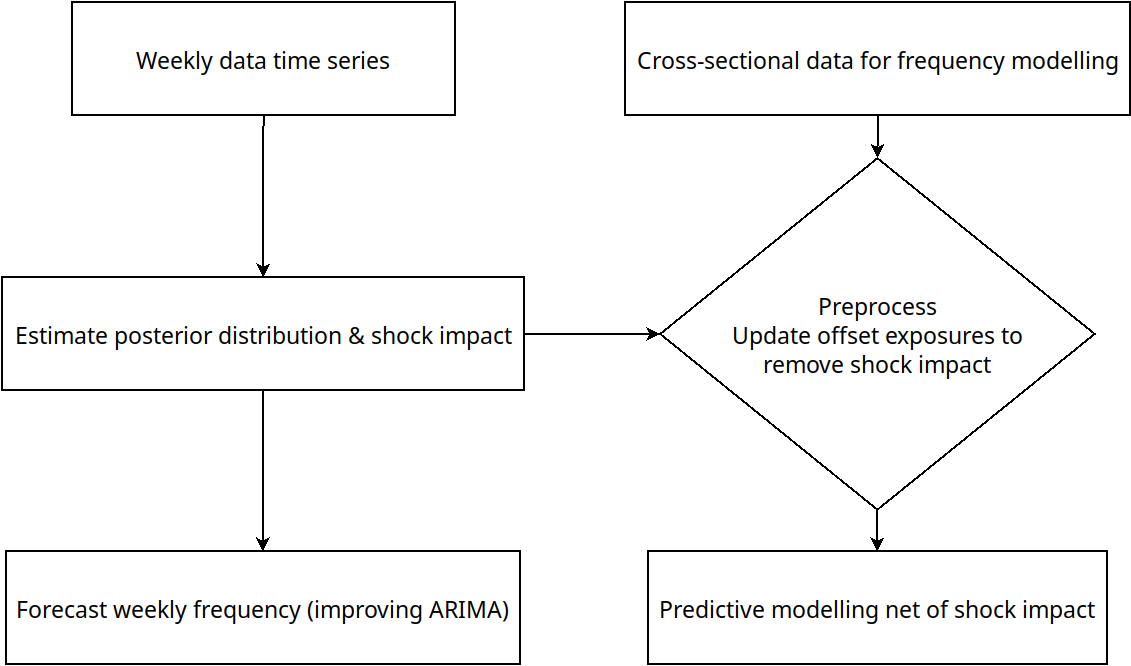
\includegraphics[width=8cm, height=5cm]{Diagrama1.png}\caption{Methodology to test the impact of a shock and filter the data afterwards.}\label{fig0}
		%\end{minipage}
  \end{figure}
	\end{center}
	

\subsection{Data}\label{data}

We observed  the weekly number of medical claims associated to a private health insurance scheme from one of the biggest companies in Spain from the beginning of 2019 to the end of 2022, by type of service, province, sex and age group. The overall monthly number of contracts was also taken into account, to control for observed trends unrelated to pandemic claiming consequences. To make the latter weekly, a linear interpolation process was performed. 

A weekly frequency count refers to the number of claims reported to the insurance company during one week. A claim refers to the use of a medical service, such as a visit to a general practitioner, a blood-test, a x-ray, a surgery, a visit to a specialist, the use of an ambulance or a treatment in an emergency room or a hospital that was covered by the insurance policy.

The insurer providing the data was affected by the enforcement of social distance measures adopted as in many other countries that actually caused a sudden decrease in the health insurance frequency of claims and the decrease was substantial due to the fact that during lock-downs in 2020 citizens reduced their normal activities and canceled preventive medical visits, while medical services were mostly dedicated to the COVID-19. Simultaneously, the insurance company portfolio initially diminished in 2020, possibly also affected by the impact of some policyholders that died during the pandemic, and grew substantially as in other European countries, something that is explained by the existence of a saturated public health system which worried many citizens who thought that they should underwrite a private health insurance on top of access to public health to protect them and their families in case of a global medical service collapse. Although private hospitals which are accessible for holders of a health insurance contract were also relatively saturated during the pandemic, COVID-19 mainly stroke public hospitals. 

The immediate impact of the COVID-19 pandemic is quantified by comparing the number of claims in the years 2019 and 2020, while the medium and long term consequences are quantified by comparing the number of claims in the years 2019, 2021 and 2022. In order to illustrate the ability of the proposed methodology to quantify the impact of the pandemic over the usage of private health services, the next section describes in detail the evolution of medical claims globally, by sex, among people over 60 years old and in the three provinces with largest Spanish cities (Madrid, Barcelona and Valencia). Additionally, some particular services of special interest are also analyzed.

In addition to what is shown here, two different scenarios were also considered regarding the definition of the post-pandemic period to be compared with the regular period (2019-01-01 to 2020-03-13) and the pandemic period (2020-03-14 to 2020-06-21). The first approach to the post-pandemic period definition is to compare the period 2019-01-01 to 2020-06-21 against the period 2020-06-22 to 2021-12-31. The second approach is to exclude the pandemic period, comparing the period 2019-01-01 to 2020-03-13 against 2020-06-21 to 2021-12-31. These results are available from the authors.

All the R code used to generate the results and figures described in the next section are available in the GitHub repository \url{https://github.com/dmorinya/XxxxBSTS} results can be reproduced with the cardiology subset. The rest of data cannot be made publicly available due to owner restrictions. All coding has been done in R software\cite{r_core_team_r_2019}, using the packages \textit{bsts}\cite{scott_predicting_nodate} and \textit{CausalImpact}\cite{brodersen_inferring_2015}. 
	
\begin{center}
  \begin{figure*}[h]
	\begin{minipage}{160mm}
    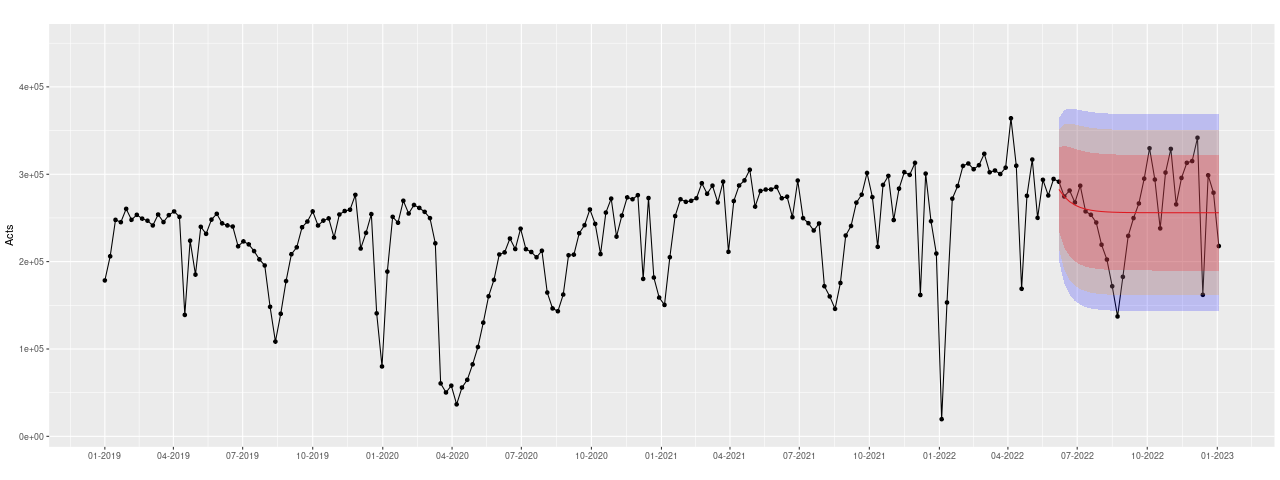
\includegraphics[width=16cm]{arima_global_prediction.png}\caption{Number of observed weekly claims (black) and ARIMA forecast for the period July-December 2022 (red), 95\% confidence bands in light blue.}\label{fig1}
	 \end{minipage}
  \end{figure*}
	\end{center}

\begin{center}
  \begin{figure*}[h]
	\begin{minipage}{160mm}
    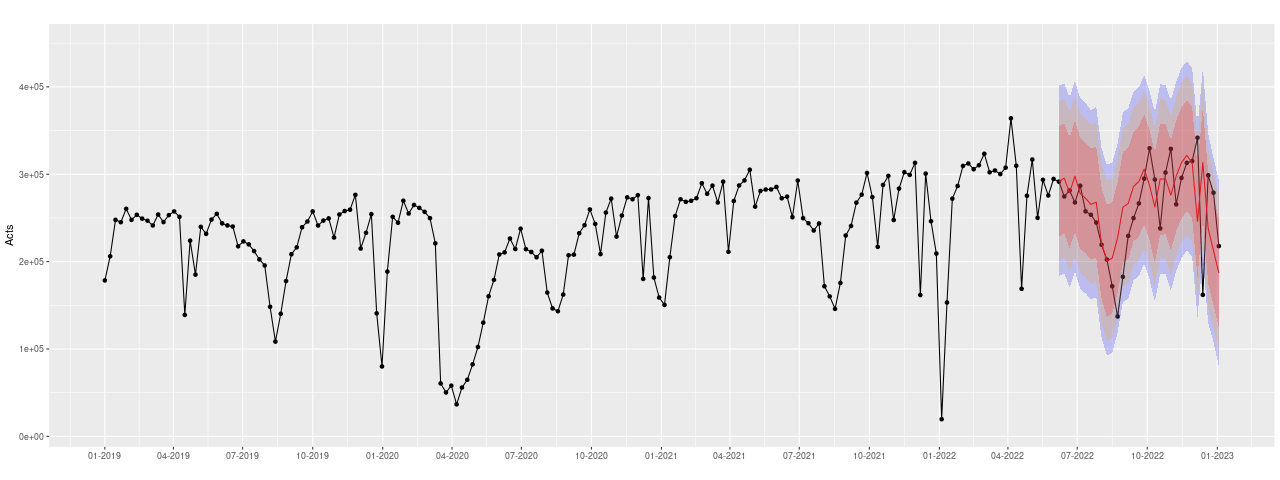
\includegraphics[width=16cm]{bsts_global_prediction.png}\caption{Number of observed weekly claims (black) and BSTS forecast for the period July-December 2022 (red), 95\% credible bands in light blue.}\label{fig2}
  \end{minipage}
  \end{figure*}
\end{center}

\section{Results}\label{results}
Although a very simplistic approach to quantifying the impact of the COVID-19 pandemic over the usage of health insurance associated services could be just to describe the reduction in claims frequency observed in 2020 with respect to  2019 and the growth observed in 2021 and 2022 also with respect to 2019, it would be complicated to use this information to forecast the future behavior of the number of claims. In our context, we could just say that in 2019 a total number of 11,754,419 claims were observed, while only 10,305,088 were observed in 2020, 13,337,053 in 2021 and 14,129,286 in 2022. Note that this figure refers to the whole portfolio of a large insurance company and the definition of a claim is any medical service provided, which can be a blood test. Overall, the global figures indicate that a decrease of 12\% was observed in 2020 and an increase of around 13\% was observed in 2021 compared to 2019, and that the increase in 2022 compared to 2019 is over 20\%. However, it is not possible to go any further from here. 

A more sophisticated approach that would allow us to get a forecast of the future behavior can be the classical ARIMA time series models, ignoring the fact that the original series is not stationary (Kwiatkowski–Phillips–Schmidt–Shin test p-value of 0.02) and it is not clear how to make it stationary using the Box-Jenkins methodology. Fitting the best ARIMA model according to the Akaike's Information Criterion (AIC) to the period January 2019 to June 2022, which is an AR(1), the produced weakly frequency of claims forecast for the period July 2022 to December 2022 is shown in Figure~\ref{fig1}. 


Figure~\ref{fig1} shows that the ARIMA based forecast is only capable of capturing the mean of the process, but at the price of large discrepancies between observed and forecasted values (RMSE of 50,094 and MAPE of 17.28\%). The forecast for the same period provided by the proposed BSTS approach in Section~\ref{methodsBSTS} is shown in Figure~\ref{fig2}.

It is clear from Figure~\ref{fig2} that the forecast produced by the proposed approach is much more accurate than that provided by the classical approach. In this case, the RMSE is around 48,388 and the MAPE is around 15.59\%, in both cases the error is lower than in the previous classical ARIMA based approach. 

Table~\ref{tab3} presents the estimated effect of the pandemic shock in the weekly time series of claims frequency observations by means of the median and 95\% credible intervals, where we also present results by groups of policy holders, geographical areas and by medical specialties. 
%{\color{red} Explicar millor què hi ha a la Taula 1}

\begin{table*}[ht]
\centering
\def\~{\hphantom{0}}
\begin{minipage}{160mm}
\caption{BSTS estimated percent median change impact of COVID pandemic and post-pandemic over the frequency usage of health insurance associated services.}
\label{tab3}
  \begin{tabular*}{\textwidth}{ccccccc}
    \Hline
    & \multicolumn{2}{c}{2019-2020} & \multicolumn{2}{c}{2019-2021} & \multicolumn{2}{c}{2019-2022}\\
    \hline
    & Difference (95\% CI) & p-value & Difference (95\% CI) & p-value & Difference (95\% CI) & p-value\\
    \hline
    Total & -12\% (-16\%, -7\%) & 0.0004 & 16\% (7.5\%, 37\%) & 0.00255 & 22\% (9.1\%, 63\%) & 0.00431\\
    \hline
    Females & -12\% (-16\%, -6.8\%) &	0.00038 & 15\% (6.3\%, 39\%) & 0.00378 & 22\% (8\%, 64\%) & 0.00591\\
    Males & -13\% (-17\%, -7.4\%) & 0.00026 & 16\% (8\%, 37\%) &	0.00237 & 22\% (11\%, 60\%) & 0.00304\\
    \hline
    Over 60 & -20\% (-24\%, -14\%) & 0.00002 & -7.2\% (-15\%, 18\%) & 0.08928 & 1\% (-11\%, 49\%) & 0.21511\\
    \hline
    Oncology &  -11\% (-17\%, -4.7\%) &	0.0025 & 8.4\% (-1.9\%, 32\%) & 0.04785 & 15\% (-0.99\%, 65\%) & 0.03075\\
    Cardiology & -10\% (-15\%, -4.8\%) & 0.00172 & 18\% (6.1\%, 39\%) & 0.00593 & 26\% (8.4\%, 61\%) & 0.0068\\
    Obstetrics & -12\% (-16\%, -7.1\%) & 0.00027 & 11\% (0.88\%, 28\%) & 0.01976 & 16\% (0.75\%, 44\%) & 0.02215\\
    Urology & -11\% (-15\%, -5.3\%) & 0.00097 & 19\% (6.7\%, 43\%) & 0.00536 & 28\% (8.8\%, 68\%) & 0.00622\\
    General medicine & 2.2\% (-2.8\%, 8.1\%) & 0.20173 & 28\% (20\%, 51\%) & 0.0001 & 48\% (37\%, 91\%) & 0.00004\\
    Osteopathy & -23\% (-27\%, -18\%) & 0.00002 & 12\% (1.8\%, 29\%) & 0.01566 & 31\% (17\%, 63\%) & 0.00301\\
    \hline
    Madrid & -16\% (-20\%, -10\%) & 0.00008 & 4.5\% (-3.6\%, 25\%) & 0.12841 & 11\% (-0.58\%, 47\%) & 0.02908\\
    Barcelona & -8.9\% (-14\%, -2.6\%) & 0.00792 & 25\% (14\%, 60\%) & 0.0003 & 33\% (16\%, 96\%) & 0.00135\\
    Valencia & -8.8\% (-13\%, -3.1\%) & 0.00487 & 29\% (19\%, 54\%) & 0.00046 & 39\% (25\%, 85\%) & 0.00034\\
    \Hline
\end{tabular*}
\end{minipage}
\end{table*}

As can be seen in Table~\ref{tab3} there is a very remarkable reduction in usage of the services associated to health insurances in 2020 compared to the previous year, except for the general medicine service, and the consequences of this reduction can be already seen in 2021 in most cases, especially in the services of urology and general medicine. The estimated 2.2\% increase observed in 2020 in general medicine (and part of the 2021 and 2022 28\% and 48\% increase respectively) can be explained because part of the COVID-19 testing was conducted under this service. Geographically, the behavior of Barcelona and Valencia is very similar in both comparisons, while Madrid shows a greater reduction in 2020 and a lower increase in 2021 and 2022, probably because Madrid has an older exposure profile, although this hypothesis cannot be confirmed with the available data since only aggregated to the national level monthly number of contracts could be obtained. The behavior of males and females is also very similar, but for people over 60 years old the reduction in 2020 is significantly greater than for the general population, and there is not an increase in 2021 (in fact, there is also a reduction of around 7\%, although it is non-significant, and a slight increase of around 1\% in 2022, again non-significant). It should be taken into account that COVID-19 associated mortality rates were much higher among this subpopulation, so it is reasonable to expect that those who old-adults (over 60 years) that survived are healthier than in the past, and therefore still using less health services than old-adults in 2019.


To illustrate how to incorporate the Bayesian estimates provided by the proposed methodology for data pre-processing, we have fitted several Poisson regression models to the number of Cardiology claims by age (30-60 / over 60) and sex (male / female). A Cardiology claim corresponds to a visit to a cardiologist. We have fitted one model per year (2019, 2020, 2021 and 2022), and a global model including data from all considered years. Additionally, we have fitted a Poisson regression model using an offset correction accounting for the global Bayesian estimates reported in Table~\ref{tab3} (-12\% for 2020, 16\% for 2021 and 22\% for 2022) and another Poisson regression model using specific Bayesian estimates for each subgroup of age and sex. The estimates yield by each of these models is reported in Table~\ref{tab1}, and the difference is obvious, especially regarding the impact of the age group parameter when using specific corrections. In this case, the last model reflects the expected claims net of the pandemic impact. This means that when all years are combined and the shock is filtered out, then the incidence in adults over 60 is 2.03 times the incidence for adult aged 30 to 60, while men's inference is 20\% higher  than women's. A year by year analysis without any shock correction would reveal lower incidence rates in general, and in particular for year 2022.


\begin{table*}[ht]
\centering
\def\~{\hphantom{0}}
\begin{minipage}{160mm}
\caption{Parameter estimates of incidence rate ratios for Poisson regression modeling the frequency of claims originating in a cardiology service (p-values correspond to testing incidence rate equals 1) for policyholder 30+ years. A correction refers to the change in exposures before estimating the Poisson regresion using the BSTS impact estimate in years 2020, 2021 and 2022 either globally, same for all individuals, or by gender/age group}
\label{tab1}
  \begin{tabular*}{\textwidth}{ccccccc}
    \Hline
    Model & $e^{\hat{\beta}_0}$ (p-value) & $e^{\hat{\beta}_\text{Sex (Male)}}$ (p-value) & $e^{\hat{\beta}_\text{Age (60+)}}$ (p-value) & Sample size\\
    \hline
    Only 2019 &  0.60 ($< 0.0001$) & 1.15 ($< 0.0001$) & 1.74 ($< 0.0001$) & 75,218 \\
    Only 2020 &  0.57 ($< 0.0001$) & 1.14 ($< 0.0001$) & 1.68 ($< 0.0001$) & 73,477 \\
    Only 2021 &  0.64 ($< 0.0001$) & 1.15 ($< 0.0001$) & 1.63 ($< 0.0001$) & 86,737 \\
    Only 2022 &  0.66 ($< 0.0001$) & 1.15 ($< 0.0001$) & 1.59 ($< 0.0001$) & 91,188 \\
    Full sample (without correction) &  0.62 ($< 0.0001$) & 1.15 ($< 0.0001$) & 1.65 ($< 0.0001$) & 
		 326,620 \\
    %Full sample (without correction and year adjusted) & -0.11 ($< 0.0001$) & 0.03 ($< 0.0001$) & 0.31 ($< 0.0001$) \\
    Full sample (with global correction) & 0.58 ($< 0.0001$)   & 1.15 ($< 0.0001$) & 1.67 ($< 0.0001$) & 
		 326,620 \\
    Full sample (with specific correction) & 0.51 ($< 0.0001$) & 1.20 ($< 0.0001$)  & 2.03 ($< 0.0001$) & 
		 326,620 \\
\Hline
\end{tabular*}
\end{minipage}
\end{table*}


\begin{table*}[ht]
\centering
\def\~{\hphantom{0}}
\begin{minipage}{160mm}
\caption{Observed and expected distribution of number of claims labelled from cardiology under each considered Poisson regression model.}
\label{tab2}
  \begin{tabular*}{\textwidth}{cccccccc}
    \Hline
    Model & 0 claims & 1 claim & 2 claims & 3 claims & 4 claims & 5 or more claims \\
    \hline
    Observed  & 150,670 & 120,040 & 38,283 & 11,499 & 3,861 & 2,267 \\ 
    Full sample (without correction) & 150,562.9 & 113,790.0 & 45,585.7 & 13,008.4 & 2,977.5 & 695.5 \\
    Full sample (with global correction) & 158,908.3 & 111,823.1 & 41,812.7 & 11,163.0 & 2,394.6 & 518.2 \\
    Full sample (with specific correction) & 163,809.8 & 108,088.0 & 40,061,1 & 11,289.5 & 2,688.8 & 682.8 \\
\Hline
\end{tabular*}
\end{minipage}
\end{table*}

As shown in Table~\ref{tab2}, the observed data is better fitted by the Poisson regression model without any correction, because the global and specific correction are modelling (with less and more detail respectively) the counterfactual that the impact of the COVID-19 pandemic is negligible. In this way, insurance companies could use the whole information in order to compare the temporal behaviour of usage series, without excluding any year. In addition, the last row of Table~\ref{tab2} refers to what the outcome distribution would have been in the absence of the pandemic shock. The full sample model with specific correction is the one than reports the expected behaviour net of the pandemic shock, and comparison with the non-corrected full model, shows how the estimated incidences impact on the final premiums.

If costs information is available, the proposed approach could be used to estimate the cost per year removing the impact of the shock. In our case, taking an average unitary cost of 50\euro{} per visit to the Cardiology service, it can be seen from Table~\ref{tab2} that the accumulated cost of Cardiology visits over the period 2019-2022 is around 12,975,500\euro{}. The actual cost per year is 3,020,850\euro{} in 2019, 2,704,550\euro{} in 2020, 3,489,900\euro{} in 2021 and 3,760,200\euro{} in 2022. Using the global adjustment, the total cost removing the impact of the pandemic can be estimated as 12,184,867\euro{}, so that implies an over cost equal to 790,633\euro{} (12,975,500\euro{}-12,184,867\euro{}). With a specific age/gender correction the estimated excess cost equals 987,116\euro{}.

Usage of other services like General Medicine was also analyzed as described in detail for Cardiology, and the results were very similar to those reported in this section.

\section{Discussion}\label{discussion}
The proposed method is capable of estimating the impact of the COVID-19 pandemic in the usage of services associated to private health insurances. Our analysis of an insurance portfolio in Spain shows that a remarkable decrease is observed in 2020 compared to the previous year, regardless of the specific service or geographic area. On the other hand, and more interestingly, our model can also estimate the posterior impact due to COVID-19 pandemic consequences, that can be translated as an increase in the usage in general (up to 29\% and 39\% in Valencia in 2021 and 2022 respectively), less clear when looking at specific services or geographic areas, probably because the increase is more subtle than the decrease during the lock-down and the time series is too short. In this sense, it would be interesting to analyze the behavior of the series when more recent data become available. As can be seen in Table~\ref{tab3}, the 2020 decrease is more relevant in less urgent services as osteopathy, while the usage of some services as cardiology or oncology could not be reduced beyond a reasonable limit.

From the insurance companies point of view, the proposed methodology offers a convenient alternative to prepare the data before implementing their pricing models for their products on the basis of realistic estimations, overcoming the most common approach to the date, which is simply to ignore the year 2020 and therefore overlooking the posterior overuse of health services due to the consequences of the COVID-19 pandemic. Also from the healthcare perspective, it is interesting to notice the differential behavior of the oldest population, as it is known that the larger health expenditure occurs a few years before decease\cite{lubitz_use_1984, scitovsky_high_2005}. 

\section{Conclusion}
When considering claim frequency data that night be affected by a pandemic shock, the identification of the impact can help understand the expected future trends. In our illustration, our results indicate little need for concern about the effects of the pandemic on claiming frequency in health insurance after 2021 for some specific groups. Old adults and some medical specialties seem to have returned to the pre-pandemic usage levels (though some services like general practitioner visits may still present unusually high frequency values). An average yearly effect was calculated for the assessment of the impact of the pandemic shock in 2021 and 2022, by service and subgroups of insureds. 

Regulators should encourage risk analysis with adequate preprocessed data when merging pre- and post- pandemic data to offset the misconception that data are comparable, that shocks can be ignored and/or they affect all individuals homogeneously. Achieving a step by step analysis like the one advocated here can lead to identify the impact of the pandemic shock and even to clarify if effects vanish or persist over time.

\backmatter

\section*{Acknowledgment}
This research was funded by Fundación MAPFRE (Becas Ignacio H. de Larramendi 2021). A.F-F. acknowledges Agencia Estatal de Investigaci\'on for the financial support IJC2020-045188I/AEI/10.13039/501100011033 and Mar\'ia Zambrano scholarship. M.G. and D.M. thank Spanish Ministry of Science and Innovation, FEDER grant PID2019-105986GB-C21 and NextGenerationEU, grant number TED2021-130187B-I00. MG gratefully thanks the ICREA Academia Program.

\bibliographystyle{plain}
\bibliography{article}

\end{document}


